\section{Feature Engineering}\label{sec:ccm}
With a collection of extracted templates from each spectrogram, feature vectors
can be constructed to distinguish between various bird species.
This is done through cross-correlation mapping, an image recognition algorithm.
A feature vector is derived from the results of cross-correlating all
templates against samples of known species.
These feature vectors are then used to train a machine learning algorithm to
classify new recordings from their spectrograms.

This section describes the mechanisms used to perform cross-correlation mapping
for feature vector construction and a short analysis of the computational
expense involved.

\subsection{Batch Processing and Result Persistency}
Once initial reductions are been made through the selection process as described
in Section~\ref{sec:template_select}, template matching is performed in batched
stages.

\subsubsection{Batching}
Further processing is batched in groups of four species, which are selected in
random order without replacement.
Each batch undergoes template matching, the results of which are stored on disk.
Once a batch is completed it is merged with previous results by cross-template
matching the new templates against the old spectrograms and the old templates
against the new spectrograms.
The new results are appended to the old feature vectors and stored on disk.

This is an effective method for dividing work into managable chunks while storing
intermediate results.
The cost analysis in the following section justifies the need for batching.

\subsubsection{Persistency}
Results are stored on disk.
This is done using the Python |Pickle| module.
Each result file is self-sufficient, as it contains all the necessary information
to classify and manipulate feature sets:
\begin{itemize}[noitemsep]
  \item Ordered list of \textbf{feature vectors} for each sample;
  \item Ordered list of numeric \textbf{labels} for each sample;
  \item Ordered list of unique \textbf{ids} for each sample;
  \item Mapping from numeric labels to real labels;
  \item List of \textbf{used templates}, in order of appearance in feature vectors.
\end{itemize}

\subsection{Template Matching}
Template matching is a method for computing the similarity of an image within
another.
We use a normalised cross-correlation method for template matching.
This mode was chosen over squared-difference and cosine-coefficient because it
has been used with good results in similar spectrogram template matching tasks
\parencite{lasseck2013}.
Normalisation is used to reduce the effect of background noise in the
spectrogram images.

The result of cross-correlation is a 2-dimensional vector with dimensions equal to
those of the target image, with values from 0 to 1. %(Figure~\ref{fig:ccm}).
Greater values indicate a higher level of correlation for the template in that
area.
This can be thought of and visualised as a heatmap of the template's correlation.

%\begin{figure}[!htb]
%  \centering
%  \begin{subfigure}[t]{0.5\textwidth}
%    \centering
%    \caption{}
%  \end{subfigure}
%  \begin{subfigure}[t]{0.5\textwidth}
%    \centering
%    \caption{}
%  \end{subfigure}
%  \begin{subfigure}[t]{0.5\textwidth}
%    \centering
%    \caption{}
%  \end{subfigure}
%  \caption{Visualisation of a cross-correlation mapping (c) of template (a) against
%  spectrogram (b)}
%  \label{fig:ccm}
%\end{figure}

Section~\ref{sec:feature_imp} discusses the mechanism and analysis of individual
feature importances.

\subsubsection{Implementation and cost}
We use Open-CV's |matchTemplate| function with the normalised CCM method.
It's implementation uses a Fourer analysis approach for improved performance over
the traditional raw statistical methods.
This works by first applying a FFT to the template and target images before
performing the cross-correlation.

Even with such optimizations, template matching takes a considerable amount of
time.
Template matching takes on average 16 minutes per spectrogram, or 0.07 seconds
per template,
given mean volume of 21941 and 34 pixels for spectrograms and templates respectively.
Considerably larger spectrograms occur often enough to add to the costs,
potentially in the order of hours.
Considering the quantity of templates being analysed, the time required quickly
amounts to days.

To gain insight into how the requirements respond to the size of a
spectrogram, a feature extraction run was performed for 80 spectrograms of
varying sizes, with 12204 total templates.
Spectrograms and templates were selected at random following the same selection
and filtering procedures described in previous sections.
Total time to completion was approximately 22 hours on the machine listed in
Appendix~\ref{app:machine}.\\

\begin{figure}[!htb]
  \centering
  \begin{subfigure}[b]{0.5\textwidth}
    \centering
    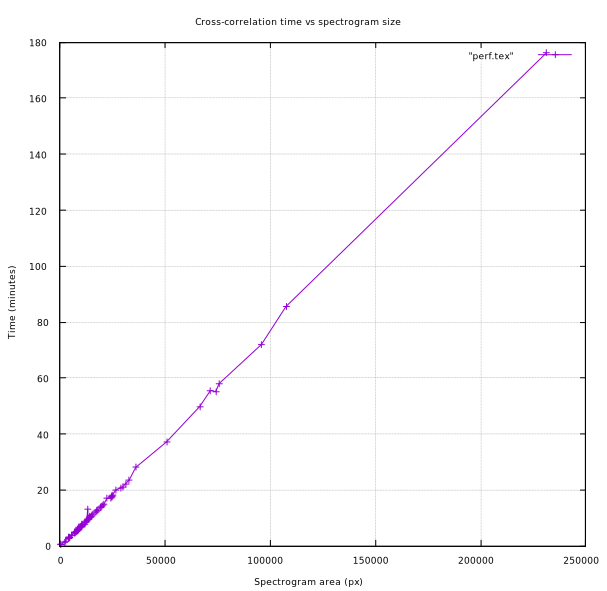
\includegraphics[width=1.0\textwidth]{ccm_time_sgram}
    \caption{}
  \end{subfigure}%
  \begin{subfigure}[b]{0.5\textwidth}
    \centering
    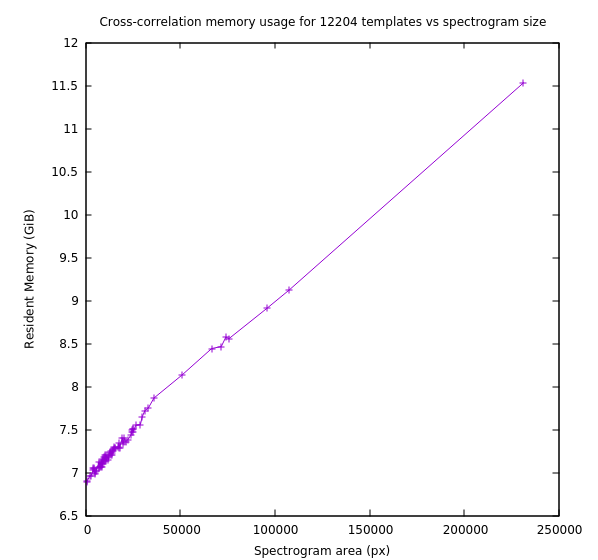
\includegraphics[width=1.0\textwidth]{ccm_mem_sgram}
    \caption{}
  \end{subfigure}
  \caption{Time (a) and resident memory (b) usages as pixel count increases for
  cross-correlation of a single spectrogram against 12204 templates}
\end{figure}

Further optimisations have been implemented.
In particular, dimensionality reduction is performed on templates and
spectrograms by blurring and reducing their size as discussed in
Section~\ref{sec:extract}.

In addition, template matching is multithreaded using Python's |multiprocessing|
module.
Spectrograms are split into even chunks equalling the number of usable CPUs on
the machine, joining results upon completion.
This cuts the cost down to approximately $1/4$ of the original time.\\

Additional optimizations could, but have not been implemented:
\begin{itemize}[noitemsep]
  \item Template matching can be confined to the general area at which the template
    was extracted.
    This is possible if the frequency bands, or image coordinates at which a
    template was extracted is stored for this purpose.
    If implemented, the search area for template matching should be increased by some
    value to account for natural or artificial deviations.

  \item Open-CV's template matching function supports on-GPU calculations.
    Doing so would result in considerable gains in speed, however this requires
    an NVIDIA CUDA device.

  \item Open-CV uses FFT.
    Fast Normalised Cross Correlation (FNCC) is a faster alternative to FFT based
    methods of template matching \parencite{briechle2001}.
    Replacing calls to an implementation which uses FNCC may result in some 
    performance gains, however an existing implementation has not been found,
    and writing one from scratch is costly without a guaranteed noticeable
    impact.
\end{itemize}

\subsection{Feature Vector Construction}
The template matching results are used to construct a feature vector for each
recording.
The feature vector of each sample therefore encodes the extent at which it's
recording contains similar characteristics to each species' song.
Feature vectors compose the training and test data for machine learning in
Chapter~\ref{cha:clf}.

The length of each feature vector is constant across all species and is equal to
the number of extracted templates.
The values of each element in the vector are derived from the template matching
results by taking the maximum value from the cross-correlation mapping.
The maxima intuitively gives us the highest matching probability for a template,
but discards information of other possible matches.
This extraction has shown promising results \parencite{fodor2013}.
